\chapter{Program Execution Monitoring}

Unicon's program execution monitoring facilities allow the user to execute a
Unicon program under the observation of one or more monitoring programs,
also written in Unicon.  This chapter begins with a brief inventory of the
monitoring architecture and its components, followed by a user's eye view of
a standard execution monitoring scenario.  The purpose of the scenario is to
characterize the execution monitoring process that is supported and to
motivate some of the features and limitations of the system.

Following the execution monitoring scenario, the functional characteristics
of each of the primary components of the execution monitoring framework are
described.  Details of the use of these components and their implementation
are presented in subsequent chapters.

\section{Monitor Architecture}

The monitoring facilities consist of the components summarized in Figure
10.1. They can be characterized in terms of their relationship to related
Unicon features.  Many of these components are general-purpose language
features that are useful independent of execution monitoring; such features,
when already present in other languages, may require modification if they
were not designed to support execution monitoring.

\begin{center}
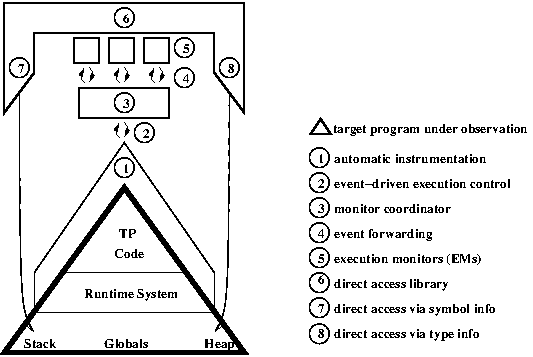
\includegraphics[width=3.1in,height=1.8in]{alamarch.png}
\end{center}

{\sffamily\bfseries Figure 10-1:}
{\sffamily The Alamo architecture}

\bigskip

\begin{list}{}{\itemsep 7pt}
\item [{\bf Dynamic loading}] --- The ability to load multiple programs
	into a shared execution environment supports
	monitor access to target program data.
	{\em Dynamic linking\/} is {\em not\/} desirable in the
	context of execution monitoring; the names in the
	monitor are distinct from those in the target program. 
	\index{dynamic loading}
\item [{\bf Synchronous execution}] --- The monitor and target program execute
	independently, but not concurrently.  This allows the monitor
	to control target program execution using a simple programming model.
	Unicon's {\em co-expression\/} data
	type supports synchronous execution of independent threads of
	execution; the mechanism is slightly extended to support the
	relationship between monitor and target program.
	\index{synchronous execution|see{coroutine}}
\item [{\bf Automatic high-level instrumentation}] --- Extensive information
	about program execution is available to the monitor from
	locations in the language runtime system that are coded to report
	significant events.  This obviates the need for control-intrusive
	techniques of obtaining information from the target program.
	It also offers higher performance than target program
	instrumentation.  The runtime system instrumentation is an
	extension and generalization of an earlier special-purpose
	monitoring facility oriented around dynamic memory allocation
	and reclamation \cite{Townsend89}.
	It also supercedes the language's built-in procedure
	tracing mechanism \cite{Griswold97}.
	\index{automatic instrumentation}
\item [{\bf Event masks}] --- Monitor control over target program
	execution is coupled with the concept of {\em filtering\/}
	\cite{Elshoff89} in a mechanism called an {\em event mask\/}.
	\index{filtering}\index{event mask}
	Event masks provide a simple, dynamic model of execution
	control that adequately meets performance requirements in
	processing the high volume of execution information.
	Events that are of no interest to the execution
	monitor are never reported and do not impose unreasonable
	execution cost.  Event masking uses a set abstraction to
	describe the execution behavior that is of interest to the monitor;
	an existing Unicon type that supports high performance set
	operations is employed to provide event masking in a manner
	that is familiar to Unicon programmers.
\end{list}


\section{Standard Execution Monitoring Scenario}

Understanding the monitoring architecture begins with a description of the
activities that it supports.  The following scenario presents the
relationship between execution monitors and target program in its
simplest form.  More sophisticated relationships between the monitor and
target program, such as running many monitors on a single
target program via a monitor coordinator, are described
in "Program Monitoring and Visualization" [Jeffery99].
In addition, the expected user and range of program behavior observable
using these monitoring facilities are characterized.

% \pagebreak

\subsection*{Definitions}

\flushleft

\includegraphics[width=0.65in,height=0.85in]{tp.png}
\vspace{-.58in}\hspace{0.5in}\parbox{27pc}{{\bf target program (TP)} ---
The target program is the Unicon program under study, a translated Unicon
executable file.
Monitoring does not require that the TP be recompiled, nor that
the TP's source code be available, although some monitors make use of
program text to present information.}\index{target program!Alamo}

\vspace{0.2in}

\flushleft
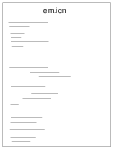
\includegraphics[width=0.65in,height=0.85in]{em.png}
\vspace{-0.85in}\hspace{0.5in}\parbox{27pc}{{\bf execution monitor (EM)} ---
An execution monitor is a Unicon program that collects and presents
information from an execution of a TP.}\index{execution monitor!Alamo}

\vspace{0.5in}

\flushleft
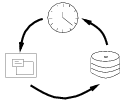
\includegraphics[width=0.6in,height=0.6in]{behave.png}
\vspace{-0.8in}\hspace{0.5in}\parbox{27pc}{{\bf program behavior} ---
Program behavior denotes the results of executing the TP.  Behavior is meant
in a general sense
that includes program output, execution time, and the precise sequence
of actions that take place during execution.}\index{program behavior}

\vspace{0.65in}

\flushleft

\includegraphics[height=0.7in]{user.png}
\vspace{-0.9in}\hspace{0.5in}\parbox{27pc}{{\bf user} --- In our standard
scenario, the user is a human capable of understanding the TP's execution
behavior.  The user must know the target language in order to make good use
of many EMs or to write a new
EM.  In general, the user need not necessarily be familiar with the TP's
source code.}\index{user!Alamo}

\vspace{0.75in}

Execution monitoring begins with a user who has questions about the behavior
of a TP (Figure ?.?). Typical questions relate to correctness or performance,
such as ``How is the result calculated?'' or ``What is taking so long?''.
Questions may be more general in nature if the user is trying to understand
how a program works, rather than to change it.

\begin{figure}[tb]
\hrule\bigskip
\centering

\hspace{0.05in}
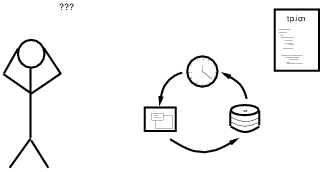
\includegraphics[height=1.7in]{scene1.png}

\caption{Monitoring starts with a user, a program, and questions.}
\medskip\hrule
\end{figure}

Answers to important questions often may be found by following the
execution as it proceeds through source language constructs, but in
high-level languages the behavior in question often depends upon the
language semantics as implemented by the language runtime system.
In Figure 4.3, {\tt iconx.c} denotes the aggregate of files that
comprise the Unicon language runtime system.\index{runtime system!Icon}
For this reason, many forms of execution monitoring
provide useful information even if the TP's source code is not available.
Figure 4.3 could be further elaborated to include behavioral
dependencies on the platform on which Unicon is implemented and run.
Such dependencies are outside the scope of this book.

\begin{figure}[tb]
\hrule\bigskip
\centering

\hspace{0.05in}
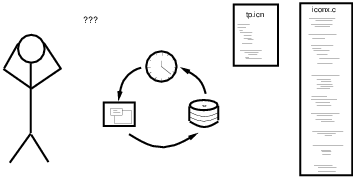
\includegraphics[height=1.7in]{scene2.png}

\caption{Behavior depends on the language, not just the program.}
\medskip\hrule
\vspace{12pt}
\end{figure}

\subsection*{Selecting or Developing Appropriate Monitors}

Rather than focusing on one monolithic EM that attempts to accommodate
all monitoring tasks, the framework advocates development of a suite
of specialized EMs that observe and present particular aspects of a
TP's behavior.  The user is responsible for selecting an appropriate
EM or set of EMs that address the user's
concerns.\index{special purpose monitors}

If no available EM can provide the needed information,
the user can modify an existing EM or write a new one.  This end user
development of execution monitors is also useful when an existing EM
provides the needed information, but it is obscured by other
information; existing EMs can be customized to a particular problem.

\subsection*{Running the Target Program}

The user runs the TP one or more times, monitored by a selection of
EMs (Figure 4.4). General-purpose EMs provide an overall impression
of program behavior.  Visualization techniques enable the presentation
of a large amount of information and abstract away detail.
\index{run!program under monitor}

\begin{figure}[tb]
\hrule\bigskip
\centering

\hspace{0.05in}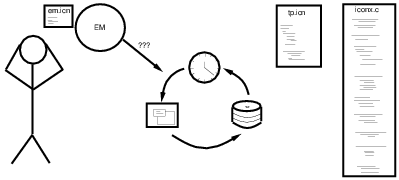
\includegraphics[width=1.7in]{scene3.png}

\caption{EMs can answer questions about TP behavior.}
\medskip\hrule
\vspace{12pt}
\end{figure}

Obtaining more specific information frequently requires that the user
interact with the EMs to control the TP's execution, either to increase
the amount of information presented during specific portions of
execution or to stop execution in order to examine details.
In order to provide this interactive control, EMs must present
execution information as it happens during the TP's execution, rather
than during a postmortem analysis phase.
\index{user!interaction}\index{execution!control}\index{analysis!runtime}
\index{analysis!post mortem}

\section{Framework Characteristics}

The preceding scenario depends on support for exploratory programming
in several areas: controlling a program's execution, obtaining execution
information, presenting large quantities of information,
and interacting with the user.  In order to support these tasks, the
framework provides synchronous shared address multitasking and an
event-driven execution control model.\index{shared address}
These features are provided by extensions to the Unicon language.


\subsection{Multitasking}

The first and most basic characteristic of the framework is an
execution model in which an EM is a separate program from the TP---a
\index{execution model!multitasking}multitasking model.
In this model the EM views the TP as a separately loaded coroutine
 \index{coroutine} \cite{Marlin80}.  The coroutine
relationship is the primary means by which EMs control TP
execution, and coroutine transfers of 
control are the primary source of execution information from a TP
(Figure ?.?).  The precise nature of the interaction between the EM and
TP (the arrows in Figure ?.?) is that of asymmetric co-expressions.

\begin{center}
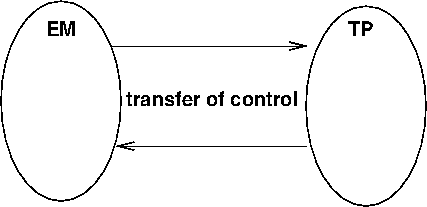
\includegraphics[width=1.7in,height=1.8in]{tpem.png}
\end{center}

{\sffamily\bfseries Figure ??-?:}
{\sffamily EM and TP are separately loaded coroutines}

\bigskip


Multitasking has the following benefits in an exploratory
programming environment: the EM and TP are independent programs, the
EM has full access to the TP, and the mechanism accommodates multiple
EMs.  These benefits are described in more detail below.


\subsubsection{Independence}

Because the EM and TP are separate programs, the TP need not be
modified or even recompiled in order to be monitored by an EM; neither
does an EM need modification or recompilation in order to be used on different
target programs.  The separation of EMs and TPs also simplifies the writing
of EMs because an EM need not be implemented as a set of callback
functions---it has its own control flow.  By definition, execution of
tasks such as EMs and TPs is synchronous.  The TP is not
running when an EM is running, and vice versa.  This synchronous
execution allows EMs and TPs to be independent without introducing the
complexity inherent in concurrent programming.
\index{independence!of EM and TP}\index{control flow}\index{callback}

Another degree of EM and TP independence is afforded by separate
memory regions; EMs and TPs allocate memory from separate heaps.
\index{memory regions!separate}\index{heap!EM separate from TP}
For this reason memory allocation in the EM does not affect the allocation
and garbage collection patterns in the TP.  Because Icon is a type-safe
language with runtime type checking and no pointer data types, EMs
and TPs cannot corrupt each others' memory by accident; only code that
contains explicit references to another program's variables and data
can modify that program's behavior.
EMs can (and some do) modify TP values in arbitrary ways; the purpose
of separate memory regions is to minimize {\em unintentional\/} data
intrusion.


\subsubsection{Access}

An address space is a mapping from machine addresses to computer memory.
\index{address space}\index{access}
Within an address space, access to program variables and data is direct,
efficient operations such as single machine instructions.  Accessing
program variables and data from outside the address space is slower and
requires operating system assistance.

In Unicon, programs such as the EM and TP reside within the same address
space.  This allows EMs to treat TP data values in the same way as
their own: EMs can access TP structures using regular Icon operations,
compare TP strings with their own, and so forth.

Because of the shared address space, the task-switching operation
needed to transfer execution between EMs and TPs is a fast,
lightweight operation.  This is important because monitoring
requires an extremely large number of task switches compared to
typical multitasking applications.\index{context switch!lightweight}
\index{task switch}


\subsubsection{Multiple Monitors and Monitor Coordinators}

Unicon's dynamic loading capabilities allow simultaneous execution of
not just a single EM and a single TP, but potentially many EMs, TPs,
and other Icon programs in arbitrary configurations.  Although uses
for many such configurations can be found, one configuration merits
special attention when many specialized EMs are available: the
execution of multiple monitors on a single TP \index{dynamic loading} (Figure 4.6).

\begin{figure}[tb]
\hrule\bigskip
\centering

\hspace{0.05in}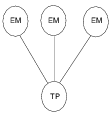
\includegraphics[height=1.1in]{multiems.png}

\caption{Multiple EMs}
\medskip\hrule
\vspace{12pt}
\end{figure}

The difficulty posed by multiple monitors is not in loading the
programs, but in coordinating and transferring control among several
EMs and providing each EM with the TP execution information it
requires.  Since EMs are easier to write if they need not be aware of
each other, this motivates construction of {\em monitor coordinators\/}
(MCs), special EMs that monitor a TP and provide monitoring services
to one or more additional EMs (Figure 4.7).  EMs receiving an MC's
services need not be aware of the presence of an MC any more than a TP
need be aware of the presence of an EM.\index{monitor coordinators}

\begin{figure}[tb]
\hrule\bigskip
\centering

\hspace{0.05in}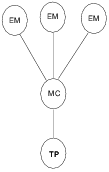
\includegraphics[height=1.7in]{mcover.png}

\caption{An execution monitor coordinator}
\medskip\hrule
\vspace{12pt}
\end{figure}

The virtual monitor interface provided by MCs makes adding a new monitor to
the system extremely easy.  A new monitor could conceivably be written,
compiled, linked, and loaded during a pause in the TP's execution. In
addition, constructing efficient MCs that provide high-level services is
another area of research that is supported within the Alamo Icon framework.
\index{virtual monitor}

\subsection{Execution Control}

The primary task of an EM is to collect data from a TP's execution.
This task poses difficult coding problems and is frequently a
performance bottleneck. The nature of the data collection facilities
available in a monitoring system also define and limit the kinds of
monitors that can be implemented.\index{data!collection}

Figure 4.8 depicts the system layers present in running a
program under the Unicon interpreter.  The TP code is executed by a
virtual machine interpreter written in C, which in turn calls C
language runtime support code to perform various language operations
\cite{Griswold86}.\index{Unicon!interpreter layers}

\begin{figure}[tb]
\hrule\bigskip
\centering

\hspace{0.05in}\includegraphics[height=2.4in]{layers.png}

\caption{Layers in the Unicon implementation}
\medskip\hrule
\vspace{12pt}
\end{figure}

Of these layers, the TP code, the virtual machine (VM), and the runtime
support code are responsible for aspects of program behavior within the
scope of this research.  The VM and the runtime system have been
extensively instrumented to produce this information for EMs at the Unicon
level without requiring instrumentation of the TP code.\index{virtual machine}

While the behavior observable from instrumentation of the VM is specific to
the Unicon interpreter and is of interest primarily to language implementors,
runtime system behavior is more general and of interest to normal
programmers.  This book is primarily concerned with monitors of runtime
system behavior.  Most of this behavior takes place even in compiled
native-code versions of the TP, with the exception of behavioral
aspects such as
runtime type checks that a compiler can avoid when static analysis
determines that they are unnecessary.

\index{instrumentation!interpreter}
This instrumentation consists of locations within the runtime
system at which control can be transferred and information reported to
the EM.  When execution proceeds through one of these points in the
runtime system, an {\em event\/} occurs.\index{event}
Many events take place during even the simplest of Icon operations.
When an EM resumes execution of the TP, it explicitly specifies what
kinds of events are to be reported; other kinds of events are not
reported. The kinds of events to be reported can be
changed dynamically each time the TP's execution is resumed (Figure 4.9).
The processing of an event
includes a test of whether the TP should transfer control to the EM
and code to perform the transfer only if the test succeeds.

Those events at which control is transferred produce {\em event reports\/}.
\index{event!report}
When an event is reported, the TP's execution is suspended
and execution commences in the program that loaded the TP---an EM.
Event reporting supports data collection in two ways: an event report
contains some information associated with the event itself, and in
addition, when the EM gains control, it can interrogate the TP's variables
and keywords for further information.  When an EM requests another
event report, the EM suspends execution and the TP's execution resumes
where it left off.

\begin{center}
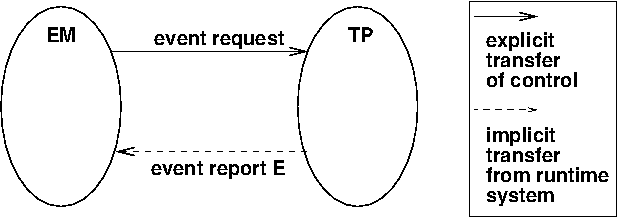
\includegraphics[width=27pc,height=1.8in]{execinf.png}
\end{center}

{\sffamily\bfseries Figure ??-?:}
{\sffamily Event-driven control of TP}
\index{event driven control}

\subsection*{Visualization Support}

Unicon's monitoring facilities explicitly support graphics output and
user interaction in EMs.
Given the amount of information associated with the execution of TP, most
EMs use graphical techniques to present abstractions of execution
information.  Since the monitor cannot in general anticipate what
information will be relevant or how to interpret it, user interaction is
crucial to the success of the monitoring process.

\subsubsection*{Simplified Graphics Programming}


Unicon includes a high-level interface to computers' graphical display
facilities; the language provides a built-in window
type.  The window and any associated window system parameters such as the
graphics drawing context and display connection are implicitly bound
together as a single value.  Programs with a primary window can
designate it as the implicit subject of all window operations.
\index{graphical user interface}\index{window!Icon type}

Graphic displays and window system software contain a variety of
resources such as colors, fonts, and images.  These resources are
allocated implicitly by the system when they are used and require
minimal attention by the user.

\subsubsection{Support for Dual Input Streams}

An EM typically has two primary input streams: the event stream from
the TP, and the input stream from the user (Figure 4.10).  Although
these two input streams are conceptually independent and may be
treated as such, for many EMs this unnecessarily complicates
the central loop that obtains event reports from TP---the EM must
also check its own window for user activity.\index{event stream!dual}
\index{input stream!dual}

\begin{center}
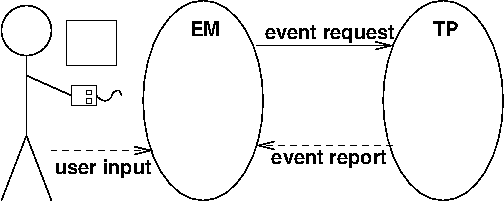
\includegraphics[width=1.5in,height=2.5in]{eventstr.png}
\end{center}

{\sffamily\bfseries Figure ??-?:}
{\sffamily Monitors have two input streams}

\bigskip


The runtime system instrumentation includes code that optionally
checks for EM input and reports it as an event by the execution
monitoring facility, instead of requiring that the EM explicitly check
the user input stream.  This simplifies EM control 
flow and improves EM performance.


\section{Monitoring Facilities Preliminary Terminology}

Before describing Unicon's monitoring execution model, a few definitions
are needed.  These definitions pertain to regions of memory referenced
by programs during execution.

\subsection{Name Spaces}
%\vspace{1.0pc}

%\noindent {\large\em Name Spaces}

%\vspace{0.25pc}
A {\em name space\/} is a mapping from a set of program source code
\index{name space}
identifiers to a set of associated memory locations \cite{Abelson85}.
Icon programs have a global name space shared across the entire
program and various name spaces associated with procedures.
Procedures each have a static name space consisting of memory
locations shared by all invocations of the procedure and local name
spaces private to each individual invocation of the procedure.

When a co-expression is created, a new local name space is allocated
for the currently executing procedure, and the current values of the
local variables are copied into the new name space for subsequent use
by the co-expression.

\subsection{Program and Co-expression State}
%\vspace{1.0pc}

%\noindent {\large\em Program and Co-expression State}

%\vspace{0.25pc}
An Icon program has an associated {\em program state\/} consisting of
\index{program state}
the memory associated with global and static name spaces, keywords,
and dynamic memory regions.  Similarly, a co-expression has an
\index{co-expression!state}
associated {\em co-expression state\/} consisting of an evaluation
stack that contains the memory used to implement one or more local
name spaces.   Co-expressions in an Icon program share access to the
program state and can use it to communicate.

\section{Tasks: An Extended Co-expression Model}

\index{task}
The central concept in MT Icon is the {\em task\/}; a task is
the execution state of a program within the Icon virtual machine
\cite{Griswold86}.  A single task called the {\em root\/} is created
when the interpreter starts execution. Additional tasks can be created
dynamically as needed.

A task consists of a main co-expression and zero or more child
co-expressions that share a program state.  At the source language
level, tasks are loaded, referenced, and activated solely in terms of
one of their member co-expressions; the task itself is implicit.

This definition of tasks is related to the concept of the same name
commonly used in operating systems and concurrent programming
languages.  It differs, however, in certain fundamental respects.
Icon is a sequential language; co-expressions in Icon provide a
synchronous coroutine execution model, not a concurrent execution
model with implicit task switching and scheduling.  Another way to
view this is that unlike other languages such as Ada, MT Icon provides
the task model as a mechanism for multitasking, but does not
predefine the policy; matters such as the scheduling algorithm used
and whether multitasking is cooperative or preemptive are
programmable at the user level.\index{algorithm!scheduling}

\index{Smalltalk!processes}
Another useful comparison can be made between Icon tasks and Smalltalk
processes.  Both provide pseudo concurrency within the context of a
sequential virtual machine.  Since Icon tasks have their own dynamic
memory regions, their presence affects each other less than
Smalltalk processes affect each other.  For example, if one task is
exhibiting thrashing heap behavior in which garbage collections are
frequent, the other tasks in the system can execute at full speed
during the portion of time in which they are running, since they
do not allocate memory out of the thrashing task's (full) heap.
This minimal effect of tasks on each others' behavior is especially
important in the domain of execution monitoring.


\subsection{Task Creation}

\index{task!creation}\index{loading!dynamic}
In MT Icon, a task can create other tasks.  The MT Icon function
\iconcode{
\> load(s, L, f1, f2, f3, i1, i2, i3)
% \> load(s, L)
}
\noindent loads an {\em icode\/} file \cite{Griswold86} specified by
the file name {\tt s}, creates a task for it, and returns a
co-expression corresponding to the invocation of the procedure
{\tt main(L)} in the loaded icode file. {\tt L} defaults to the empty list.
Unlike conventional Icon command-line argument lists, the argument list
passed to {\tt load()} can contain values of any type, such as procedures,
lists, and tables in the calling task.

The task being loaded is termed the {\em child\/} task, while
the task calling {\tt load()} is termed the {\em parent\/}.  The
collection of all tasks forms a tree of parent-child relationships.
\index{parent!task}
\index{child!task}
\index{tree!of tasks}

{\tt f1}, {\tt f2}, and {\tt f3} are files to use as
{\tt \&input}, {\tt \&output}, and {\tt \&error} in the loaded
task; they default to those of the loading task.  {\tt i1}, {\tt i2},
and {\tt i3} supply initial region sizes in bytes for the
task's block, string, and stack memory areas, respectively. 
The defaults for these sizes may be specified by environment variables
% {\tt i1} and {\tt i2} default to 65000, while {\tt i3} defaults
% to 20000 (the defaults may be changed by the environment variables
{\tt BLKSIZE}, {\tt STRSIZE}, and {\tt MSTKSIZE}.

\subsection{Running Other Programs}

\index{run!loaded program}
A co-expression created by {\tt load()} is activated like any other
co-expression. When activated with the {\tt @} operator, the child
task begins executing its main procedure. Unless it suspends or
activates {\tt \&source},
the child task runs to completion, after which control is returned
to the parent.  Chapter 6 presents an alternative means of executing
a child in which the parent retains control over the child as it executes.

\subsubsection*{An Example}
%\vspace{1.0pc}

%\noindent {\large\em An Example}

%\vspace{0.25pc}
This default behavior is illustrated by the program {\tt seqload},
which loads and executes each of its arguments (string names of
executable Icon programs) in turn.  In this program the variable
{\tt arguments} is a list of strings passed into the Icon program from
the operating system.  Each of these strings (extracted from the list
using the element generation operator, {\tt !}) is passed in turn to
{\tt load()}.  {\tt load()} reads the code for each argument and
creates a task in which to execute the loaded program; the tasks are
then executed one by one by the co-expression activation operator,
{\tt @}.  This is ordinary Icon code; there is nothing special about
this example except the semantics of the {\tt load()} function and the
independent execution environment (separate global variables, heaps,
and so forth) that {\tt load()} provides to each task.

The child programs can also be used as standalone Icon applications, or can
be loaded into other multitasking Icon programs.  This approach contrasts
with the use of shell scripts or a series of calls to {\tt system()} to run
a sequence of Icon programs.

\iconcode{
	\# seqload.icn \\
	procedure main(arguments) \\
\>	    every @load(!arguments) \\
	end
}

For example, if three Icon programs whose executable files are named
{\tt translate}, {\tt assemble}, and {\tt link} are to be run in
succession, the command
\iconcode{
seqload translate assemble link
}
\noindent executes the three programs without reloading the
interpreter for each program.




\section{Data Access}

Although tasks have separate sets of global variables and keywords,
they reside in the same address space and can share data.
\index{global variable}\index{task}
This data access applies to all first-class data objects in Icon, such
as procedures and co-expressions.  Values can be transmitted from
task to task through {\tt main()}'s argument list,
by means of explicit intertask access functions, or by
use of event monitoring facilities described later on.

\subsection{Access Through Task Argument Lists}
%\vspace{1.0pc}

%\noindent {\large\em Access Through Task Argument Lists}

%\vspace{0.25pc}
The following program takes its first argument to be an Icon program
to load and execute as a child, sorts its remaining arguments, and
supplies them to the child program as its command-line arguments
({\tt pop()} and {\tt sort()} are Icon built-in functions that extract
the first list element and sort elements, respectively):

\iconcode{
	procedure main(arguments) \\
\>	   @load(pop(arguments), sort(arguments)) \\
	end
}

Argument lists allow more sophisticated data transfers; the {\tt seqload} 
example presented earlier can be extended to transmit arbitrary
structures between programs using argument lists in the following
manner.  As in {\tt seqload}, each string naming an executable Icon
program is passed into {\tt load()}, and the resulting task is
activated to execute the program.  In this case, however, any result
that is returned by one of the programs is assigned to local variable
{\tt L} and passed to the next program in the list via the second
argument to {\tt load()}.

\iconcode{
     \# seqload2.icn \\
     procedure main(arguments) \\
\>	every program := !arguments do \\
\>\>	   L := @load(program, L) \\
     end
}

The net effect of {\tt seqload2.icn} is similar to a UNIX pipe, with
an important difference: Arbitrary Icon values can be passed from
program to program through the argument lists.
This capability is more interesting in substantial multipass tools
such as compilers, where full data structures can be passed along from
tool to tool instead of writing out text encodings of the structures
to a file.

\subsection{Inter-task Access Functions}
%\vspace{1.0pc}

%\noindent {\large\em Intertask Access Functions}

%\vspace{0.25pc}
Several of Icon's built-in functions are enhanced under Unicon
\index{access!variable}\index{variable@{\tt variable()}}
to provide inter-task access to program data.  For example, the
{\tt variable()} function in Unicon takes a co-expression value as an
optional second argument denoting the task from which to fetch the named
variable.  When called with this second argument, {\tt variable()} is
useful for assigning to or simply reading values from another task's
variables.  In this modified version of the {\tt seqload} example, the
parent task initializes each child task's {\tt Parent} global
variable (if there is one) to refer to the parent's {\tt \&main}
co-expression.  A child task can then use this variable to determine
whether it is being run standalone or under a parent task.
Inter-program access through the {\tt variable()} function is also
useful in inspecting values, especially at intermediate points during
the monitored execution of a TP.

\iconcode{
     \# seqload3.icn \\
     procedure main(arguments) \\
\>	every arg := !arguments do \{ \\
\>\>	   Task := load(arg) \\
\>\>	   variable(\"Parent\", Task) := \&main \\
\>\>	   @Task \\
\>\>	   \} \\
	end
}

In addition to MT's extensions of existing functions, several new
functions have been added.  These facilities are useful in execution
monitoring and are used in examples in Unicon's ipl/mprogs directory
and described in ``Program Monitoring and
Visualization''. Some of
the intertask access functions used in examples are listed in Figure
?.?.  In these functions, parameter {\tt C} refers to a co-expression
that may be from a task other than the one being executed.  In proper
Icon style, functions that are said to {\em generate} values can produce
more than one result from a given call.
\index{function!execution monitoring}\index{generator!function}
\index{access!functions}

\begin{figure}[t]
\hrule\bigskip
\centering

\begin{tabular}{|ll|} \hline
{\bf\tt cofail(C)}      & transmit failure to {\tt C}. \\
{\bf\tt fieldnames(r)}  & generate fieldnames of record {\tt r}. \\
{\bf\tt globalnames(C)} & generate the names of {\tt C}'s global
variables. \\
{\bf\tt keyword(s, C)} & produces keyword {\tt s} in {\tt C}. \\
	& Keywords are special global variables that have \\
	& special semantics in certain language facilities.\\
{\bf\tt localnames(C,i)} & generates the names of {\tt C}'s local variables,\\
	& {\tt i} calls up from the current procedure call. \\
{\bf\tt paramnames(C,i)} & generates the names of {\tt C}'s parameters. \\
{\bf\tt staticnames(C,i)} & generates the names of {\tt C}'s static variables. \\
{\bf\tt structure(C)} & generates the values in {\tt C}'s block
region, or heap. \\
	 & The heap holds structure types such as lists and tables. \\
{\bf\tt variable(s,C,i)} & produces variable named {\tt s}, interpreted {\tt i} levels\\
	& up within {\tt C}'s procedure stack. \\
\hline
\end{tabular}

\caption{Unicon interprogram access functions.}
\medskip\hrule
\end{figure}





\section{Terminology}

The terminology used in discussing execution monitoring relates to
events and the linguistic features associated with them.

\subsection*{Events}

The primary linguistic concept added in order to support execution \index{event}
monitoring is an {\em event\/}.  An event is the smallest unit of
execution behavior that is observable by a monitor.  In practice, an
event is the execution of a point of instrumentation in the code
called a {\em sensor\/} \cite{Ogle90} \index{sensor}
that is capable of transfering control to the monitor.

\index{instrumentation}
This definition limits events to those aspects of program behavior
that are instrumented in the language runtime system or the program
itself.  The event model is only as useful or general as is the
instrumentation that extracts program information.  If instrumentation does
not exist for an aspect of program behavior of interest, it is often
possible to monitor the desired behavior by means of other events. 
In the present implementation, for example, no instrumentation exists
for file input and output.  If an EM wishes to monitor I/O behavior, it
can monitor function and operator events and act on those functions
and operators that relate to input and output.  A similar example
involving the monitoring of Icon's built-in string scanning functions
is presented in [Jeffery99]

The Unicon definition of event also differs from that of many
monitoring systems, in which the term event refers to the basic unit
of information {\em received\/} by the monitor \cite{Bates89}.  The
distinction is that in the Unicon definition, events occur whether
they are monitored or not, and each event may or may not be observed
by any particular monitor.  This definition is useful in the MT
Icon environment, in which EMs are not coupled with the
instrumentation and multiple EMs can observe a TP's execution.

\subsection*{Event Codes and Values}

From the monitor's perspective, an event has two components: an
\index{event!code}\index{event!value}
{\em event code\/} and an {\em event value\/}.  The code is
generally a one-character string describing what type of event
has taken place.  For example, the event code {\tt C} denotes a
procedure call event.  Event codes all have associated symbolic
constants used in program source code.  For example the mnemonic for a
procedure call event is {\tt E\_Pcall}.  These constants are available
to programmers as part of a standard event monitoring library
described below.\index{E\_Pcall@{\tt E\_Pcall}}

The event value is an Icon value associated with the event.  The
nature of an event value depends on the corresponding event code.
For example, the event value for a procedure call event is an
Icon value designating the procedure being called, the event value for
a list creation event is the list that was created, the event value
for a source location change event is the new source location, and so
forth.  Event values can be arbitrary Icon structures with pointer
semantics; the EM accesses them just like any other source language
value.\index{access!structure}

\subsection*{Event Reporting and Masking}

The number of events that occurs during a program execution is
extremely large---large enough to create serious performance problems
in an interactive system.  Most EMs function effectively on a
small fraction of the available events; the events that an EM uses
are said to be {\em reported\/} to the EM.  An {\em event report\/}
results in a transfer of control from the TP to the EM.  Efficient
support for the selection of appropriate events to report and the
minimization of the number of event reports are primary concerns.
\index{event!report}

Unicon supports {\em dynamic event masking\/} based on event codes,
a dynamic variation of the filter concept found in most event-based
monitoring systems
\cite{Bates89} \cite{Elshoff89}.\index{event!mask}
Event masking allows the monitor to specify which
events are to be reported and to change the specification at runtime.
When the program being monitored starts execution, the monitor selects
a subset of possible event codes from which to receive its first
report.  The program executes until an event occurs with a selected
code, at which time the event is reported.  After the monitor has
finished processing the report, it transfers control back to the
program, again specifying an event mask.  Dynamic event masking
enables the monitor to change the event mask in between event reports.

The use of one character strings as event codes has a more practical
value than its mnemonic merit: it allows sets of codes to be
efficiently and easily manipulated at the Icon level by the {\em cset\/}
(character set) data type.  Csets are represented internally by bit
vectors, so a cset membership test is very efficient compared to
Icon's more generic set data type, whose membership test is a hash
table lookup.\index{cset!event mask}\index{character set!event mask}

When an event report transfers control from TP to EM, the two components of
the event are supplied in the Icon keywords {\tt \&eventcode} and {\tt
\&eventvalue}, respectively.\index{event!code}\index{event!value}
As discussed earlier, these
keywords are special global variables that are given their values by the
Icon runtime system during an event report, rather than by explicit user
assignment.  The monitor then
can act upon the event based on its code, display or manipulate its value,
etc.


\section{Obtaining Events Using {\tt evinit}}

A standard library called {\tt evinit} provides EMs with
a means of obtaining events.  Programs wishing to use the
standard library include a link declaration such as {\tt link
evinit}.\index{evinit library}
\index{library procedures!monitor}
In addition, monitors include a header file named {\tt evdefs.icn}
to obtain the symbolic names of the event codes.
\index{evdefs.icn@{\tt evdefs.icn}}

%\subsection*{Setting Up an Event Stream}
\vspace{1pc}

\addcontentsline{toc}{subsection}{\protect\numberline{6.2.1}{Setting Up an Event Stream}}
\noindent {\large\em 6.2.1 \ \ \ Setting Up an Event Stream}

\vspace{0.25pc}
\noindent
An EM first sets up a source of events; the act of monitoring then
\index{event!source}
consists of a loop that requests and processes events from the TP.
\index{EvInit@{\tt EvInit()}}
Execution monitoring is initialized by the procedure
{\tt EvInit(x{\em [,input,output,error]\/})}.  If {\tt x} is a string, it is
used as an icode file name in a call to the Unicon function {\tt load()}.
If {\tt x} is a list, its first argument is taken as the icode file name
and the rest of the list is passed in to the loaded function as the
arguments to its main procedure.
{\tt EvInit()} assigns the loaded
TP's co-expression value to EM's {\tt \&eventsource} keyword.
The {\tt input}, {\tt output}, and {\tt error} arguments are files
used as the loaded program's standard files.

EMs generally call the library procedure {\tt EvTerm()} when they complete,
passing it their main window (if they use one) as a parameter.
\index{EvTerm@{\tt EvTerm()}}
{\tt EvTerm()} informs the user that execution has completed and allows the
final screen image to be viewed at the user's leisure, waiting for the user to
press a key or mouse button in the window and then closing it.

The typical EM, and all of the EMs presented as examples in this
book, follow the general outline:\index{outline!of an EM}
\index{skeleton!of an EM} \index{template!of an EM}

%%%% \pagebreak
\iconcode{
     \$include \"evdefs.icn\" \\
     link evinit \\
     procedure main(arguments) \\
\>	EvInit(arguments) $\mid$ stop(\"can't initialize monitor\") \\
\>	\# ... initialization code, open the EM window \\
\>	\# ... event processing loop (described below) \\
\>	EvTerm() \\
     end
}
\noindent This template is generally omitted from program examples for
the sake of brevity.

%\subsection*{\tt EvGet()}
\vspace{1pc}

\addcontentsline{toc}{subsection}{\protect\numberline{6.2.2}{{\tt EvGet()}}}
\noindent {\large\em 6.2.2 \ \ \ {\tt EvGet()}}

\vspace{0.25pc}
Events are requested by an EM using the function {\tt EvGet(mask)}.
\index{EvGet@{\tt EvGet()}}
{\tt EvGet(mask)} activates the co-expression value of the keyword 
{\tt \&eventsource} to obtain an event whose code is a member of the
cset {\tt mask}.
{\tt mask} defaults to {\tt \&cset}, the universal set indicating all events
are to be reported.
The TP executes until an event report takes place; the resulting code and
value are assigned to the keywords {\tt \&eventcode} and {\tt \&eventvalue}.
{\tt EvGet()} fails when execution terminates in TP.

%\subsection*{Event Masks and Value Masks}
\vspace{1pc}

\addcontentsline{toc}{subsection}{\protect\numberline{6.2.3}{Event Masks and Value Masks}}
\noindent {\large\em 6.2.3 \ \ \ Event Masks and Value Masks}

\vspace{0.25pc}
\noindent
{\tt EvGet()} allows a monitor the flexibility to change event masks each
\index{value masks}
time the event source is activated.  Another function that sets event masks
is {\tt eventmask()}.  {\tt eventmask(C,c)} sets the event mask of the task
owning co-expression C to the cset value given in {\tt c}.

Event masks are the most basic filtering mechanism in Alamo, but there are
situations where they are not specific enough.  For example, instead of
handling events for all list operations, you may want events only for
specific lists.  This situation is supported by the concept of {\em value
masks}.  A value mask is an Icon set or cset whose members are used to
filter events based on their {\tt \&eventvalue}, just as an event mask
filters based on the {\tt \&eventcode}.  You may specify a different value
mask for each event code.  Value masks for all event codes are supplied in a
single Icon table value whose keys map event codes to corresponding value
masks.  This table is passed as an optional second parameter to {\tt EvGet()}
or third parameter to {\tt eventmask()}.  Note that no value mask filtering
is performed for event codes that are not key in the value mask.  Note also
that value masks persist across calls to {\tt EvGet()}. They are replaced
when a new value mask is supplied, or disabled if a non-table is
passed as the value mask parameter.

There is one special case of value masks that receives extra support in
Icon: virtual machine instructions.
\index{virtual machine!instruction}
Requesting an event report for the execution of the next virtual
machine instruction is performed by calling {\tt EvGet()} with an event
mask containing {\tt E\_Opcode}.  VM instructions occur
extremely frequently; dozens of them can occur as a result of the
execution of a single line of source code.  Consequently, performance
is severely affected by the selection of all VM instruction events.

However, a particular instruction or small set of instructions
may be of interest to a monitor.  In that case, the EM need not
receive reports for all instructions.  The function {\tt opmask(C, c)}
allows EM to select a subset of virtual machine instructions given by
{\tt c} in {\tt C}'s task.  Subsequent calls to {\tt EvGet()} in
which {\tt E\_Opcode} is selected reports events only for the VM
instructions designated by~{\tt c}.
\index{E\_Opcode@{\tt E\_Opcode}}

The event values for {\tt E\_Opcode} are small non-negative integers.  They
fall in a limited range ($<$ 256), which is what allows a cset
representation for them.  Symbolic names for individual virtual machine
instructions are defined in the include file {\tt opdefs.icn}.
{\tt opmask(C, c)} is equivalent to:

% \pagebreak
\iconcode{
   t := table() \\
   t[E\_Opcode] := c \\
   eventmask(C, , t)
}
\vspace{-1.5pc}

\section{Instrumentation in the Icon Interpreter}

This section describes the instrumentation used by Unicon to produce
events at various points in the runtime system.  Significant points in
interpreter execution where transfer of control might be warranted are
explicitly coded into the runtime system with tests that result in
transfer of control to an EM when they succeed.  When execution reaches
one of these points, an event occurs.  Events affect the execution
time of the TP; execution is either slowed by a test and branch
instruction (if the event is not of interest to the EM), or stopped
while the event is reported to the EM and it processes information.
Minimizing the slowdown incurred due to the presence of monitoring
instrumentation has been a focus of the implementation.

There are several major classes of events that have been instrumented
in the Unicon intepreter.  Most of these events correspond to explicit
elements within the source code; others designate actions performed
implicitly by the runtime system that the programmer may be unaware of.
A third class of event that has been instrumented supports user
interaction with the EM rather than TP behavior.
\index{event!categories}

%\subsection*{Explicit Source-Related Events}
\vspace{1pc}

\addcontentsline{toc}{subsection}{\protect\numberline{6.3.1}{Explicit Source Related Events}}
\noindent {\large\em 6.3.1 \ \ \ Explicit Source Related Events}

\vspace{0.25pc}
\noindent
The events that relate behavior observable from the source code are:

\begin{list}{}{\itemsep 7pt} % was itemize
\item [{\bf Program location changes}] --- Source code locations are
	reported in terms of line numbers and columns.
\item [{\bf Procedure activity}] --- There are events for procedure calls,
	returns, failures, suspensions,
	and resumptions.  In addition to these explicit forms of
	procedure activity, events occur for implicit removals of
	procedure frames.
\item [{\bf Built-in functions and operations}] --- Events that correspond
	to Icon built-ins describe many areas of behavior from numeric and
	string operations to structure accesses	and assignments.
	Like procedures, events are produced for function and operator calls,
	returns, suspensions, resumptions, and removals.
\item [{\bf String scanning activity}] --- Icon's pattern matching
	operations include scanning environment
	creation, entry, change in position, and exit.  To obtain
	a complete picture of string scanning, monitors must
	observe these events along with the built-in functions
	related to string scanning.
\end{list}

%\subsection*{Implicit Runtime System Events}
\vspace{1pc}

\addcontentsline{toc}{subsection}{\protect\numberline{6.3.2}{Implicit Runtime System Events}}
\noindent {\large\em 6.3.2 \ \ \ Implicit Runtime System Events}

\vspace{0.25pc}
\noindent
Events that depict important program behavior observed within the runtime
system include:

\begin{list}{}{\itemsep 7pt} % was itemize
\item [{\bf Memory allocations}] --- Memory is allocated from the
	string and block regions in the heap.  Allocation events
	include size and type information.
	This instrumentation is based on earlier instrumentation added to Icon
	\index{memory monitor}
	for a memory monitoring and visualization system \cite{Townsend89}.

\item [{\bf Garbage collections}] --- The storage region being
	\index{garbage collection}
	collected (Icon has separate regions for strings and data
	structures), the memory layout after compaction, and the
	completion of garbage collection are reported by several events.
\item [{\bf Type conversions}] --- In Icon, automatic conversions are
	performed on parameters	to functions and
	operators.  Information is available for conversions
	attempted, failed, succeeded, and found to be unnecessary.
	\index{type!conversion}\index{conversion!type|see{type, conversion}}
\item [{\bf Virtual machine instructions}] --- Icon's semantics may be
	defined by a sequence of instructions executed by the Icon virtual
	machine \cite{Griswold86}.  The program can receive events for
	\index{virtual machine!instruction}
	all virtual machine instructions, or an arbitrary subset.
\item [{\bf Clock ticks}] --- The \index{clock tick} passage of CPU time
	is indicated by a clock tick.
\end{list}

% \subsection{Monitor Interaction Events}

Most EMs, except completely passive visualizations and profiling
tools, provide the user with some degree of control over the
monitoring activity and must take user interaction into account.
\index{execution control}
For example, the amount of detail or the rate at which the monitor
information is updated may be variables under user control.  Since
an EM's user input occurs only as often as the user presses keys or
moves the mouse, user interaction is typically far less frequent than
events in TP.  Even if no user input occurs, polling for user input
may impose a significant overhead on the EM because it adds code to
the central event processing loop.\index{polling}

In order to avoid this overhead, the event monitoring instrumentation
includes support for reporting user activity in the EM window as part
of the TP's event stream.\index{user!input}
Monitor interaction events are requested by
the event code {\tt E\_MXevent}.  An example of the use of monitor
interaction events is presented further in this chapter in the section
entitled ``Handling User Input''.  A complete list of event codes
is presented in Appendix ?? in order to indicate the extent of the
instrumentation.\index{E\_MXevent@{\tt E\_MXevent}}


\section{Artificial Events}

\index{event!artificial}
As described above, the Unicon co-expression model allows
interprogram communication via explicit co-expression activation or
implicit event reporting within the runtime system.
{\em Artificial events\/} are events produced by explicit 
Icon code; they can be viewed at the language level as co-expression
activations that follow the same protocol as implicit events,
assigning to the keyword variables {\tt \&eventcode} and
{\tt \&eventvalue} in the co-expression being activated.

\index{event!virtual}\index{event!pseudo}
There are two general categories of artificial events, {\em virtual events\/}
meant to be indistinguishable from implicit events and {\em pseudo events\/}
that convey control messages to an EM.  Virtual events are generally
used either to produce event reports from manually instrumented
locations in the source program, to simulate event reports, or to pass
on a real event from the primary EM that received it to one or
more secondary EMs.  Pseudo events, on the other hand, are used for
more general inter-tool communications during the course of monitoring,
independent of the TP's execution behavior.

%\subsection*{Virtual Events Using {\tt event()}}
\vspace{1pc}

\addcontentsline{toc}{subsection}{\protect\numberline{6.4.1}{Virtual Events Using {\tt event()}}}
\noindent {\large\em 6.4.1 \ \ \ Virtual Events Using {\tt event()}}

\vspace{0.25pc}
\noindent
The function {\tt event(code, value, recipient)} sends
\index{event()@{\tt event()}}
a virtual event report to the co-expression {\tt recipient}, which
defaults to the {\tt \&main} co-expression in the parent of the
current task, the same destination to which implicit events are
reported.

There are times when a primary EM wants to pass on its events to a
secondary EM.  An example would be an event transducer that sits
in between the EM and TP, and uses its own logic to
determine which events are reported to EM with more precision
than is provided by the masking mechanism.  A transducer might just as
easily report extra events with additional information
it computes, in addition to those received from TP. 
A more substantial application of virtual events is a monitor
coordinator, an EM that coordinates and produces events for
other monitors.  Such a tool is presented in [Jeffery99]

%\subsection*{Pseudo Events for Tool Communication}
\vspace{1pc}

\addcontentsline{toc}{subsection}{\protect\numberline{6.4.2}{Pseudo Events for Tool Communication}}
\noindent {\large\em 6.4.2 \ \ \ Pseudo Events for Tool Communication}

\vspace{0.25pc}
\noindent
EMs generally have an event processing loop as their central
\index{tool communication}\index{communication!tool}\index{pseudo events}
control flow mechanism.  The logical way to communicate with such a
tool is to send it an event.  In order to distinguish a message from a
regular event report, the event code must be distinguishable.  In the
monitoring framework, this is achieved simply by using an event code
other than a one-letter string, such as an integer.  Since not all EMs
handle such events, they are not delivered to an EM unless it passes a
non-null second argument (the ``value mask argument'') to {\tt EvGet()},
such as {\tt EvGet(mask,~1)}.

The framework defines a minimal set of standard pseudo events, which
well-behaved EMs should handle correctly [Jeffery99].  Beyond this
minimal set, pseudo events allow
the execution monitor writer to explore communication between EMs as
another facility to ease programming tasks within the monitoring
framework.


\section{Monitoring Techniques}

Monitors generally follow a common outline and use a common set of
facilities, which are described below.

\subsection*{Anatomy of an Execution Monitor}

The execution monitoring interface uses
\index{monitor!template} \index{monitor!anatomy}
a form of {\em event driven\/} programming: \index{event driven programming}
the central control flow of EM is a loop that executes the TP
for some amount of time and then returns control to EM
with information in the form of an event report.  The
central loop of an EM typically looks like:

% \pagebreak %%%%

\iconcode{
     while EvGet(eventmask) do \\
\>	case \&eventcode of \{ \\
\>\>	   \# a case clause for each code in the event mask \\
\>\>	   \}
}

Event-driven programming is more commonly found in programs that
employ a graphical user interface, where user activity dominates
control flow. Because monitoring employs a programming paradigm that
has been heavily studied, many coding techniques developed for
graphical user interface programming, such as the use of callbacks
\cite{Clark85}, are applicable to monitors. Several of the example EMs
in the IPL use a callback model to take advantage of a
higher-level monitoring abstraction available by means of a library
procedure.

\subsection*{Handling User Input}

An EM that handles user input could do so by polling the window system
after each event in the main loop: \index{user!input}

\iconcode{
     while EvGet(eventmask) do \{ \\
\>	case \&eventcode of \{ \\
\>\>	   \# a case clause for each code in the event mask \\
\>\>	   \} \\
\>	\# poll the window system for user input \\
\>	\}
}

\noindent If the events being requested from the TP are relatively
infrequent, this causes no great problem.  However, the more frequent
the event reports are, the more overhead is incurred by this approach
relative to the execution in TP.  In typical EMs, polling for user
events may slow execution from an imperceptible amount to as much as 15
percent.   Relative frequency for different types of events varies
wildly; it is discussed in [Jeffery99].

Since the slowdown is a function of the frequency of the event reports and
not just the cost of the polling operation itself, techniques such as
maintaining a counter and polling once every {\em n\/} event reports still
impose a significant overhead.  In addition, such techniques reduce the
responsiveness of the tool to user input and therefore reduce the user's
control over execution.

Monitor interaction events, presented earlier in this chapter,
address this performance issue by allowing user input to be supplied
via the standard event stream produced by {\tt EvGet()}.
\index{EvGet@{\tt EvGet()}}
\index{E\_MXevent@{\tt E\_MXevent}}
Since the {\tt E\_MXevent} event occurs far less
frequently than other events, it makes sense to place it last in the
case expression that is used to select actions based on the event
code.  Using this feature, the main loop becomes: 

\iconcode{
     while EvGet() do \\
\>	case \&eventcode of \{ \\
\>\>	   \# other cases update image to reflect the event \\
\>\>	   E\_MXevent: \{ \\
\>\>\>	      \# process user event \\
\>\>\>	      \} \\
\>\>	   \}
}
 
{\tt EvGet()} reports pending user activity immediately when it is
available; the control over execution it provides is comparable to
polling for user input on each event.


%\subsection*{Querying the Target Program for More Information}
\vspace{1pc}

\addcontentsline{toc}{subsection}{\protect\numberline{6.5.3}{Querying the Target Program for More Information}}
\noindent {\large\em 6.5.3 \ \ \ Querying the Target Program for More Information}

\vspace{0.25pc}
\noindent
After each event report, EMs can use Unicon's intertask data access
\index{access!functions}
functions to query TP for additional information, such as the values
of program variables and keywords.  The access functions can be used
in several ways, such as

\begin{itemize}
\item applying a predicate to each event report to make monitoring
	more specific,
\item {\em sampling\/} execution behavior not reported by events by
	polling the TP for information unrelated to the event reports
	\cite{Ogle90}, or \index{sampling}
\item presenting detailed information to the user, such as the
	contents of variables.
\end{itemize}


\section{Some Useful Library Procedures}

As mentioned in Section 6.2, several library procedures are useful
in EMs.  This section presents those library procedures that are
included in the {\tt evinit\/} library.
\index{evinit@{\tt evinit}}

Location decoding and encoding procedures are useful in processing 
location change event values, but they are also useful in other monitors
in which two-dimensional screen coordinates must be manipulated.
Besides program text line and columns, the technique can variously be
applied to individual pixels, to screen line and columns, or to screen
grid locations in other application-specific units.

In addition, various EMs use utility procedures.  Figure 6.2 lists the
library procedures that are used in this book.

\begin{figure}[t]
\hrule\bigskip
\centering

\begin{tabular}{|ll|} \hline
procedure  & returns or computes \\
{\tt evnames(s)} & converts event codes to text descriptions and vice versa\\
{\tt evsyms()} & two-way table mapping event codes to their names \\
{\tt typebind(w,c)} & table mapping codes to color coded Clones for {\tt w}\\
{\tt opnames()} & table mapping VM instructions to their names \\
{\tt location()} & encodes a two dimensional location in an integer \\
{\tt vertical()} & y/line/row component of a location \\
{\tt horizontal()} & x/column component of a location \\
{\tt prog\_len()} & number of lines in the source code for TP \\
{\tt procedure\_name()} & name of a procedure \\
{\tt WColumns()} & window width in text columns \\
{\tt WHeight()} & window height in pixels \\
{\tt WRows()} & window height in text rows \\
{\tt WWidth()} & window width in pixels \\
\hline
\end{tabular}

\caption{Additional library procedures for monitors.}
\medskip\hrule
\end{figure}


\section{Typical Evolution of a Visualization Tool}

Many visualization tools can be written by adapting a similar existing tool;
in fact, many of the simple visualizations described later in this book are
intended as starting points for such programs.  Because program
visualization is still a relatively undeveloped area, however, there are
still frequent situations where a new monitor is written to visualize a new
behavior of interest.  In such a situation, the monitor writer gets to work
from scratch.

While every programmer may approach the task of writing a visualization tool
differently, we found over time that a consistent approach has been useful
for a wide range of tools.  Our method is incremental and reflects the view
that the monitoring task is predominant over the graphics programming task
in constructing such tools.  We present the sequence of tasks here in order
to encapsulate this experience.  Following the approach is no guarantee that
the end product will be successful, but it may simplify for the reader the
order in which various components are best assembled.

%\subsection*{Generate Log Files}
\vspace{1pc}

\addcontentsline{toc}{subsection}{\protect\numberline{6.8.1}{Generate Log Files}}
\noindent {\large\em 6.8.1 \ \ \ Generate Log Files}
\nopagebreak

\vspace{0.25pc}
\noindent
\index{log file}
The initial emphasis should be to characterize precisely the behavior of
interest.  Program execution behavior is expressed in terms of a stream of
events; example code for handling them
was given earlier in this chapter.  A prose description of the behavior of
interest may be useful, but a state machine or grammar that describes the
event sequences that constitute the behavior of interest is a more useful
formalization.

Some behavior will not be described adequately by a regular or context-free
sequence of events.  In particular, some monitors may have to examine
variables and check complex conditions within the program being observed, in
order to find the behavior of interest.  For these reasons, the ultimate
formal preparation prior to writing the visualization code is to produce a
fully operational monitor that observes the desired event sequences and
writes the relevant events to a logfile.  This text-only monitor can be tested
to establish confidence in it before starting the task of graphics coding.

%\subsection*{Depict the Log Files}
\vspace{1pc}

\addcontentsline{toc}{subsection}{\protect\numberline{6.8.2}{Depict the Log Files}}
\noindent {\large\em 6.8.2 \ \ \ Depict the Log Files}

\vspace{0.25pc}
\noindent
Once a monitor that observes the correct behavior is written, the primary
graphic design and programming can be performed.  In the absence of an
obvious metaphor, it is possible to start from the same information that
was being written to the logfiles and animate it as a sequence of points or
more complex objects plotted along a Cartesian or radial axis.

\subsection*{Scale to Handle Real Problems}

For most monitors, multiple forms of scaling are necessary in order to
\index{scale}
produce a usable tool from the initial graphic design.  Traditional scaling
involves multiplying coordinates by a scaling factor in order to ensure
that the plotted coordinates do not go outside the visible area of the
window.  Other forms of scaling begin the conversion from graphs to
visualizations. This includes condensation of multiple events down to
individual output operations, and of multiple graphic outputs onto
a shared space in the window.  Several iterations of scaling may be applied
as needed.

\subsection*{Focus on Behaviors of Interest}

Scaling often leads to enough loss of detail that the user cannot see the
\index{focus}
behaviors of interest, they can only see the big picture.  For cataclysmic
events of interest, the monitor can help the user notice behaviors of
interest by drawing attention to them using flashing lights, sound, or
whatever. For more nebulous or tenuous situations, the monitor's goal should
be to show enough information for users to decide whether something needs
further investigation.  Showing more details for atypical behavior is a good
starting point.  To show more details, the tool requires more screen space.
Log scales or hyperbolic or fisheye views allocate conspicuously more screen
space to some elements than to others.

% \pagebreak

\subsection*{Add User-Directed Navigation}

Ultimately, the user will need to be able to specify objects on the
\index{navigation}
visualization for which additional detailed information is of interest.
Adding navigation may be more difficult than rendering the graphics in the
first place.  The visualization tool will need to perform hit tests to
determine which object the user is selecting.  This requires a data
structure that provides access to on-screen entities, and efficiency may
become an issue for very large numbers of objects.  This task typically
leads to the additional graphics programming required to produce detailed
views of objects of interest.


\section{Conclusions}

Unicon includes linguistic facilities to exploit the instrumentation
available within Icon's runtime system.  By adding language-level support,
exploratory development of execution monitors is possible using the Icon
lanuage instead of Icon's implementation language, C.  Writing a monitor
consists of writing an ordinary application in a rapid prototyping language,
instead of low-level systems programming that requires intimate knowledge of
the Icon implementation.
The key concepts introduced for Unicon's event monitoring facilities are
events, event reports, event codes and values, and event masks.  Monitors
also make use of a standard monitoring library and Icon's graphics
facilities.

While the details presented in this chapter are specific to Icon, the results
are not.  The success of Unicon's monitoring framework in facilitating
construction of new execution monitoring tools is not limited in
applicability to Icon---it suggests that if high-quality execution
monitors are a priority, designers of high-level languages should consider
incorporating monitoring support in the language design rather than leaving
it to the ad-hoc devices of some post-implementation afterthought.  This
support should consist of more than just symbol table information for
source variable names.
